A la hora de implementar el control PD se encontraron varios problemas en la estimación de la derivada (\autoref{eq:derivada discreta}). 

\begin{figure}[H]
    \centering
    
\includegraphics[width=0.8\textwidth]{img/PD/PD-Derivada ruidosa.png}
    \caption{Error y su derivada.}
    \label{fig:derivada ruidosa}
\end{figure}

La \autoref{fig:derivada ruidosa} muestra el error medido por el sensor ultrasónico y su derivada calculada según la Ecuación \ref{eq:derivada discreta}. Puede notarse que esta última no es representativa de la derivada real del error, por lo que implementar un control PD con esta estimación resultaría problemático. El ruido intrínseco en la medición del sensor ultrasónico es la causa de la imprecisión en el cálculo de la derivada, por lo que para solucionar este problema sería necesario cambiar el sensor. Sin embargo, se encontró que, sin solucionar el problema de fondo, puede corregirse la estimación de la derivada para hacerla más representativa del comportamiento real del error.

En primer lugar, puede notarse en la \autoref{fig:derivada ruidosa} que la derivada oscila alrededor del 0. Este comportamiento se explica analizando la \autoref{eq:derivada discreta}. Nótese que el primer término de la misma $\left(\frac{2}{T_s}(e_k - e_{k-1})\right)$ podría resultar despreciable comparado con el segundo ($D_{k-1}$). Si esto ocurriera, en el instante $k$ se tendría que $D_k \approx - D_{k-1}$, con lo cual esta situación se propagaría al instante $k + 1$ y a los siguientes. Esto es, en efecto, lo que se observa en la \autoref{fig:derivada ruidosa}, en la que la derivada oscila entre $-2000$ y $2000$ aproximadamente. Esto explica por qué cuando el error se mantiene constante la derivada no es cero.

En segundo lugar, puede destacarse que valores tan elevados de la derivada resultan ilógicos. Si la derivada en el instante $k$ fuera realmente $2000\,\sfrac{\text{cm}}{\text{s}}$, el carrito se estaría moviendo a esa velocidad, o, lo que es equivalente, el carrito habría recorrido los \SI{40}{\cm} de la barra en tan solo un intervalo de muestreo. 

En base a estas dos observaciones se propone modificar el cálculo de la derivada de la siguiente forma: en primer lugar, ya que el sensor ultrasónico tiene una resolución mínima de $0,3\,$cm, si el cambio en el error es menor a esta cantidad, debe considerarse que no hay cambio real y forzar a que la derivada en ese instante sea nula. En segundo lugar, si el cambio en la medición del error es demasiado grande, debe considerarse que la medición es inválida y no se debe actualizar la derivada. De esta forma, se tienen dos umbrales, \texttt{UMBRAL\_INF} y \texttt{UMBRAL\_SUP}. Si $e_k - e_{k-1} < \text{\texttt{UMBRAL\_INF}}$, el cambio en el error es demasiado pequeño y se considera que $D_k = 0$. Si $e_k - e_{k-1} > \text{\texttt{UMBRAL\_SUP}}$ se considera que la medición es inválida y la derivada mantiene su valor.

\begin{figure}[H]
    \centering
    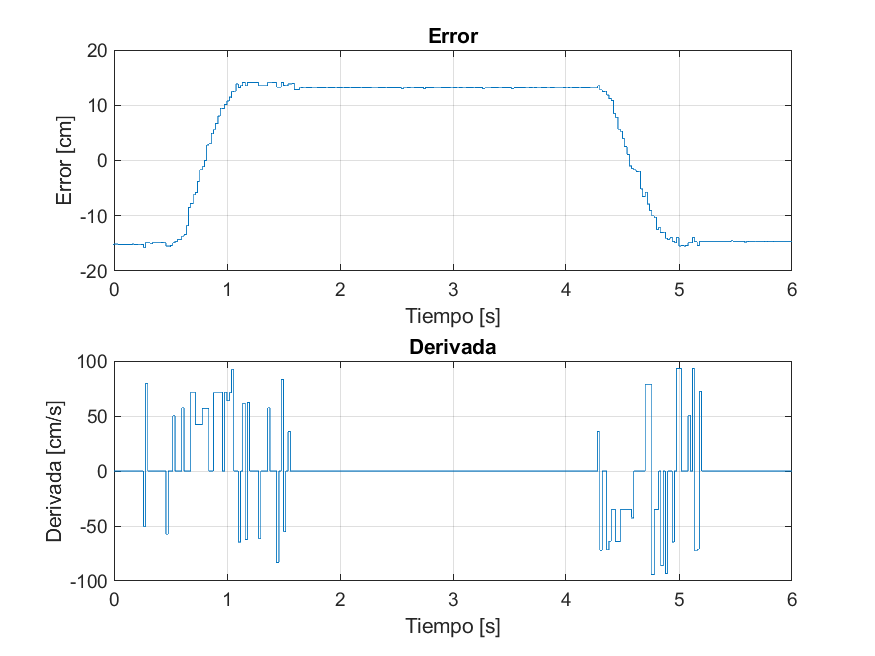
\includegraphics[width=0.8\textwidth]{img/PD/PD-derivada mejorada.png}
    \caption{Nueva estimación de la derivada}
    \label{fig:derivada mejorada}
\end{figure}

La Figura \ref{fig:derivada mejorada} muestra cómo queda la estimación de la derivada con estas limitaciones. Puede notarse que cuando el error es aproximadamente constante la derivada se mantiene en cero y que la misma es menos sensible al ruido de medición. Sin embargo, todavía presenta evidentes imperfecciones. Los umbrales elegidos fueron $\texttt{UMBRAL\_INF} = 0,3\,\text{cm}$ y $\texttt{UMBRAL\_SUP} = \SI{1}{\cm}$.

Similar al método seguido en las secciones anteriores, se eligieron $k_p = 2,5$ y $k_d = 0,1$ de forma tal de resolver el compromiso entre estabilidad y velocidad de respuesta de forma satisfactoria. En este caso, además, se buscó evitar la saturación de la acción de control. 

\begin{figure}[H]
    \centering
    
\includegraphics[width=0.8\textwidth]{img/PD/PD-Bode de L.png}
    \caption{Diagrama de Bode de $L(s)$.}
    \label{fig:PD-bode}
\end{figure}

\begin{figure}[H]
    \centering
    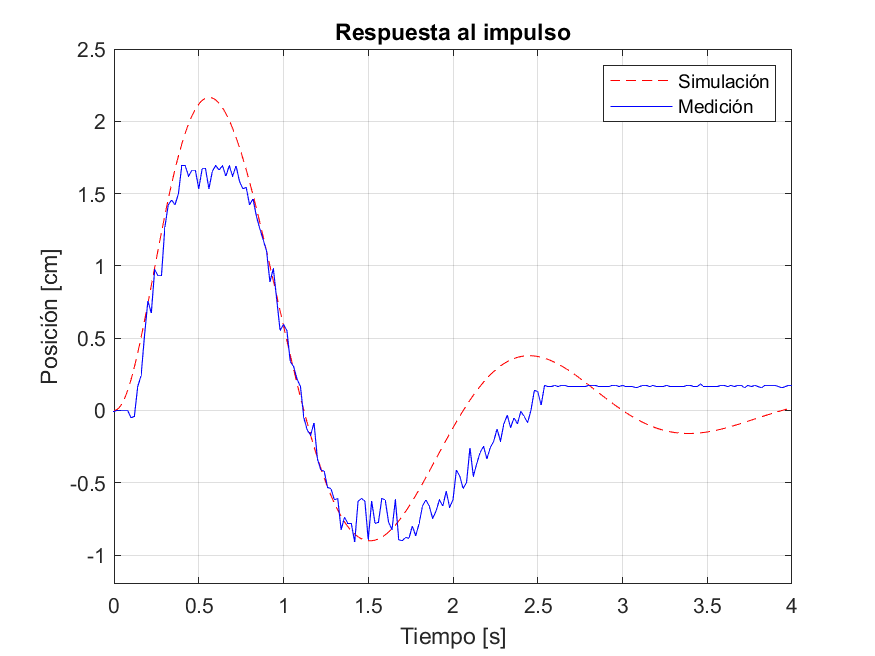
\includegraphics[width=0.8\textwidth]{img/PD/PD-Respuesta al impulso.png}
    \caption{Respuesta al impulso del control PD.}
    \label{fig:PD-respuesta al impulso}
    
\end{figure}

\begin{figure}[H]
    \centering
    
\includegraphics[width=0.8\textwidth]{img/PD/PD-Acción de control(escalón).png}
    \caption{Acción de control de la respuesta al impulso.}
    \label{fig:PD-acción de control impulso}
\end{figure}

\begin{figure}[H]
    \centering
    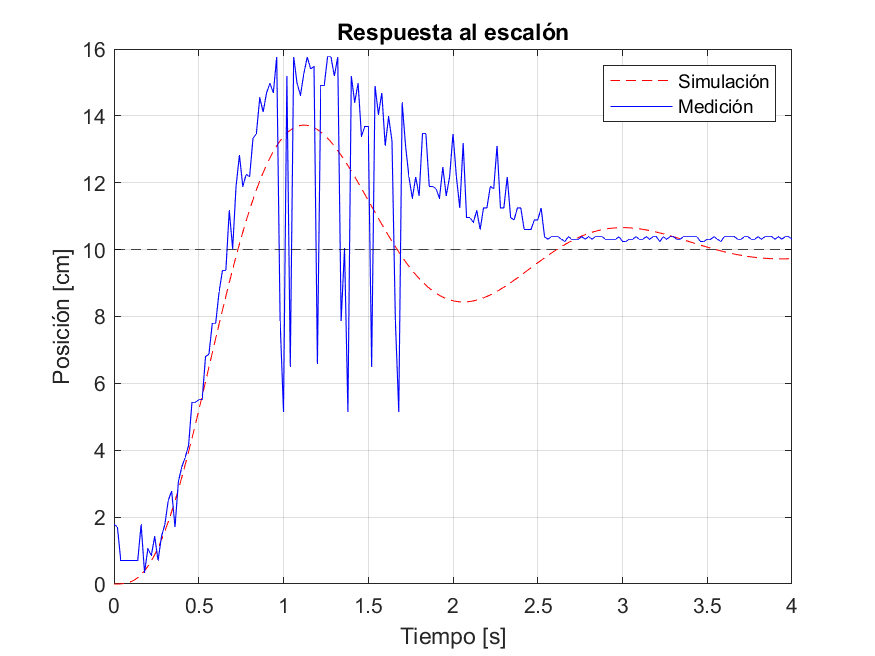
\includegraphics[width=0.8\textwidth]{img/PD/PD-Respuesta al escalón.png}
    \caption{Respuesta al escalón del control PD.}
    \label{fig:PD-respuesta al escalón}
\end{figure}

\begin{figure}[H]
    \centering
    
\includegraphics[width=0.8\textwidth]{img/PD/PD-Acción de control(escalón).png}
    \caption{Acción de control de la respuesta al escalón.}
    \label{fig:PD-acción de control escalón}
\end{figure}

Se observa tanto en la Figura \ref{fig:PD-respuesta al impulso} como en la \ref{fig:PD-respuesta al escalón} que la posición medida y la estimada son similares en algunos puntos y presentan evidentes diferencias en otros. Además, la posición logra estabilizarse en la referencia satisfactoriamente. Por otro lado, tanto en la Figura \ref{fig:PD-acción de control impulso} como en la \ref{fig:PD-acción de control escalón} se observa que se alcanzó el objetivo de no saturar la acción de control, cuyos límites se indican en línea negra rayada.